% =============================================================================
% cover-embedded-projekt.tex – Cover für Selection Panel Firmware
% =============================================================================
% Kompilieren: xelatex cover-embedded-projekt.tex
% Erzeugt: cover-embedded-projekt.pdf (für \coverimage in main.tex)
% =============================================================================
\documentclass[tikz,border=0pt]{standalone}

% -----------------------------------------------------------------------------
% SCHRIFTEN (identisch mit techdoc.cls)
% -----------------------------------------------------------------------------
\usepackage{fontspec}
\defaultfontfeatures{Ligatures=TeX}

\setmainfont{TeX Gyre Pagella}
\setsansfont{TeX Gyre Heros}
\setmonofont[Scale=0.85]{TeX Gyre Cursor}

% -----------------------------------------------------------------------------
% FARBEN (identisch mit techdoc.cls)
% -----------------------------------------------------------------------------
\usepackage{xcolor}

% Primärfarben
\definecolor{ArduinoTeal}{HTML}{00979D}
\definecolor{ArduinoDark}{HTML}{005C5F}
\definecolor{RaspberryRed}{HTML}{C51A4A}

% Statusfarben
\definecolor{SuccessGreen}{HTML}{75A928}
\definecolor{WarningOrange}{HTML}{D97706}

% Neutrale Farben
\definecolor{MutedText}{HTML}{4A5568}
\definecolor{CodeBg}{HTML}{F8FAFC}
\definecolor{CodeFrame}{HTML}{C8D2DC}

% -----------------------------------------------------------------------------
% TIKZ-BIBLIOTHEKEN
% -----------------------------------------------------------------------------
\usetikzlibrary{shapes, arrows.meta, positioning, calc, decorations.pathreplacing}

% -----------------------------------------------------------------------------
% STILE
% -----------------------------------------------------------------------------
\begin{document}
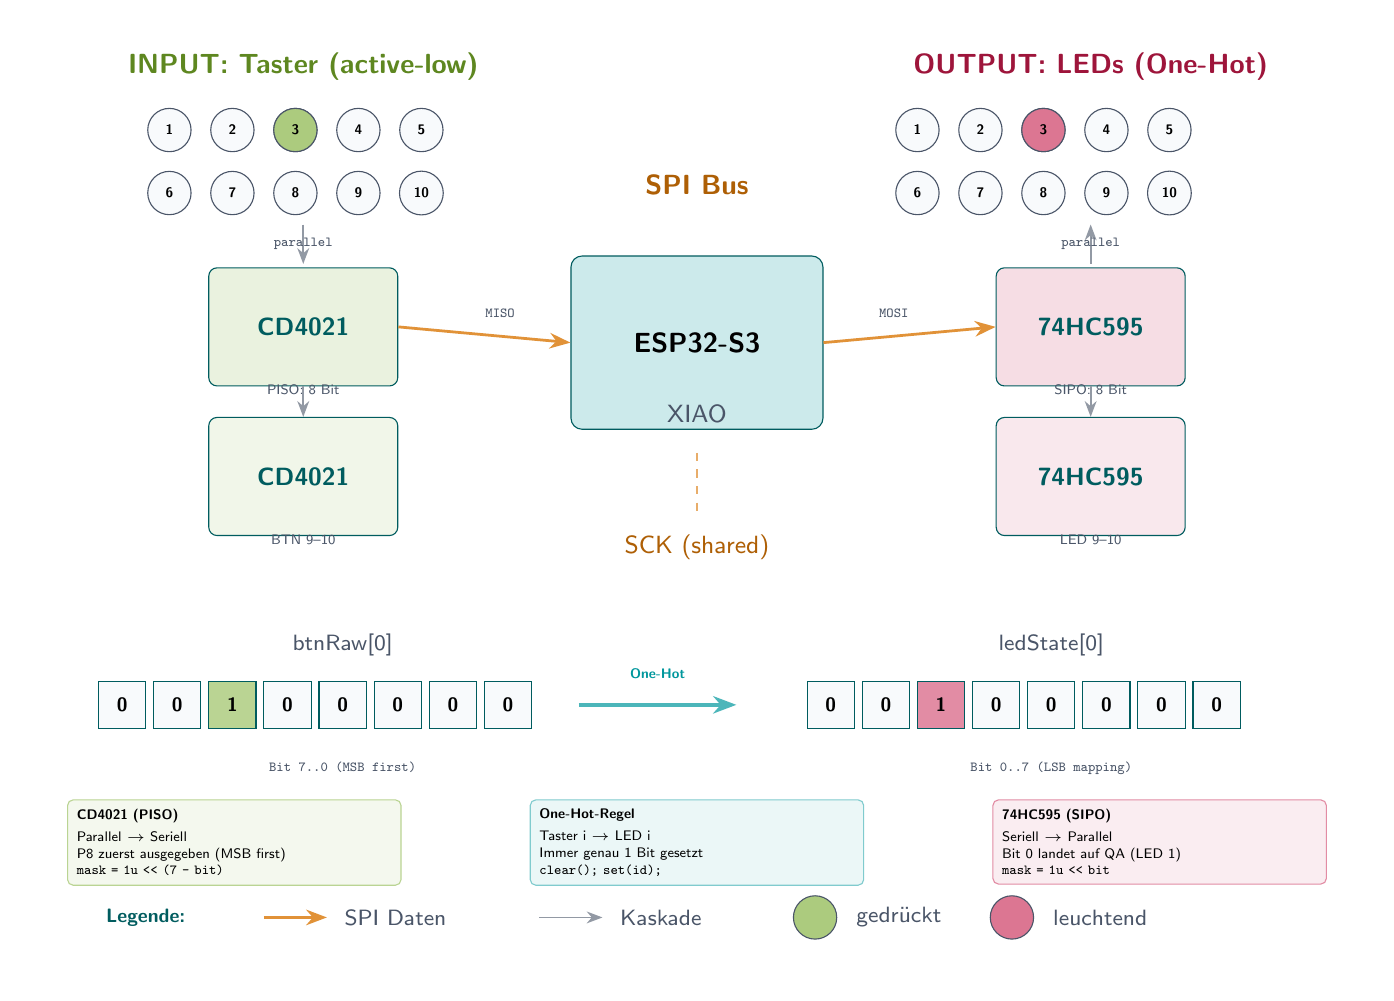
\begin{tikzpicture}[
  % === GRUNDSTILE ===
  chip/.style={
    draw=ArduinoDark,
    fill=#1,
    minimum width=2.4cm,
    minimum height=1.5cm,
    rounded corners=3pt,
    font=\sffamily\bfseries\small
  },
  chip/.default=white,
  % Mikrocontroller
  mcu/.style={
    draw=ArduinoDark,
    fill=ArduinoTeal!20,
    minimum width=3.2cm,
    minimum height=2.2cm,
    rounded corners=4pt,
    font=\sffamily\bfseries
  },
  % Taster
  button/.style={
    draw=MutedText,
    fill=#1,
    circle,
    minimum size=0.55cm,
    font=\sffamily\bfseries\tiny
  },
  button/.default=CodeBg,
  % LED
  led/.style={
    draw=MutedText,
    fill=#1,
    circle,
    minimum size=0.55cm,
    font=\sffamily\bfseries\tiny
  },
  led/.default=CodeBg,
  % Bit-Box
  bitbox/.style={
    draw=ArduinoDark,
    fill=#1,
    minimum width=0.6cm,
    minimum height=0.6cm,
    font=\sffamily\bfseries\scriptsize
  },
  bitbox/.default=ArduinoTeal!30,
  % Infobox
  infobox/.style={
    draw=#1!50,
    fill=#1!8,
    rounded corners=2pt,
    font=\sffamily\tiny,
    text width=4cm,
    align=left
  },
  infobox/.default=ArduinoTeal,
  % Labels
  lbl/.style={
    font=\sffamily\footnotesize,
    color=MutedText
  },
  bitlbl/.style={
    font=\ttfamily\tiny,
    color=MutedText
  },
  % Pfeile
  dataarrow/.style={
    draw=ArduinoTeal!70,
    line width=1pt,
    ->,
    >=Stealth
  },
  spiarrow/.style={
    draw=WarningOrange!80,
    line width=1pt,
    ->,
    >=Stealth
  },
  chainarrow/.style={
    draw=MutedText!60,
    line width=0.6pt,
    ->,
    >=Stealth
  }
]

% =============================================================================
% HINTERGRUND
% =============================================================================
\fill[white] (-1,-4) rectangle (16,8);

% =============================================================================
% LINKE SEITE: TASTER + CD4021
% =============================================================================

% Überschrift
\node[font=\sffamily\bfseries, color=SuccessGreen!80!black] 
      at (2.5,7.5) {INPUT: Taster (active-low)};

% Taster-Reihe (10 Stück, 2 Zeilen à 5)
\foreach \i in {1,...,5} {
  \node[button=CodeBg] (btn\i) at (\i*0.8, 6.7) {\i};
}
\foreach \i in {6,...,10} {
  \pgfmathtruncatemacro{\col}{\i-5}
  \node[button=CodeBg] (btn\i) at (\col*0.8, 5.9) {\i};
}

% Highlight: Taster 3 gedrückt
\node[button=SuccessGreen!60] at (2.4, 6.7) {3};

% CD4021 Chips
\node[chip=SuccessGreen!15, text=ArduinoDark] (cd1) at (2.5,4.2) {CD4021};
\node[font=\sffamily\tiny, color=MutedText] at (2.5,3.4) {PISO: 8 Bit};

\node[chip=SuccessGreen!10, text=ArduinoDark] (cd2) at (2.5,2.3) {CD4021};
\node[font=\sffamily\tiny, color=MutedText] at (2.5,1.5) {BTN 9--10};

% Pfeile Taster → CD4021
\draw[chainarrow] (2.5,5.5) -- (2.5,5);
\node[bitlbl] at (2.5,5.25) {parallel};

% Kaskade CD4021
\draw[chainarrow] (cd1.south) -- (cd2.north);

% =============================================================================
% MITTE: ESP32-S3
% =============================================================================

\node[mcu] (esp) at (7.5,4) {ESP32-S3};
\node[font=\sffamily\small, color=MutedText] at (7.5,3.1) {XIAO};

% SPI-Bus Beschriftung
\node[font=\sffamily\bfseries, color=WarningOrange!80!black] at (7.5,6) {SPI Bus};

% 74HC595 Chips (definieren vor Pfeilen)
\node[chip=RaspberryRed!15, text=ArduinoDark] (hc1) at (12.5,4.2) {74HC595};
\node[font=\sffamily\tiny, color=MutedText] at (12.5,3.4) {SIPO: 8 Bit};

\node[chip=RaspberryRed!10, text=ArduinoDark] (hc2) at (12.5,2.3) {74HC595};
\node[font=\sffamily\tiny, color=MutedText] at (12.5,1.5) {LED 9--10};

% MISO: CD4021 → ESP32
\draw[spiarrow] (cd1.east) -- (esp.west);
\node[bitlbl, above] at (5,4.2) {MISO};

% MOSI: ESP32 → 74HC595
\draw[spiarrow] (esp.east) -- (hc1.west);
\node[bitlbl, above] at (10,4.2) {MOSI};

% SCK (gemeinsam)
\draw[WarningOrange!60, line width=0.8pt, dashed] (7.5,2.6) -- (7.5,1.8);
\node[font=\sffamily\small, color=WarningOrange!80!black] at (7.5,1.4) {SCK (shared)};

% =============================================================================
% RECHTE SEITE: 74HC595 + LEDs
% =============================================================================

% Überschrift
\node[font=\sffamily\bfseries, color=RaspberryRed!80!black] 
      at (12.5,7.5) {OUTPUT: LEDs (One-Hot)};

% Kaskade 74HC595
\draw[chainarrow] (hc1.south) -- (hc2.north);

% LED-Reihe (10 Stück, 2 Zeilen à 5)
\foreach \i in {1,...,5} {
  \node[led=CodeBg] (led\i) at (\i*0.8+9.5, 6.7) {\i};
}
\foreach \i in {6,...,10} {
  \pgfmathtruncatemacro{\col}{\i-5}
  \node[led=CodeBg] (led\i) at (\col*0.8+9.5, 5.9) {\i};
}

% Highlight: LED 3 leuchtet (One-Hot)
\node[led=RaspberryRed!60] at (11.9, 6.7) {3};

% Pfeile 74HC595 → LEDs
\draw[chainarrow] (12.5,5) -- (12.5,5.5);
\node[bitlbl] at (12.5,5.25) {parallel};

% =============================================================================
% DATENFLUSS-VISUALISIERUNG (Bytes)
% =============================================================================

% Taster-Byte (MSB first) - LINKS
\node[lbl, anchor=south] at (3,-0.1) {btnRaw[0]};
\node[bitlbl, anchor=north] at (3,-1.2) {Bit 7..0 (MSB first)};
\foreach \i/\val/\col in {0/0/CodeBg, 1/0/CodeBg, 2/1/SuccessGreen!50, 3/0/CodeBg, 4/0/CodeBg, 5/0/CodeBg, 6/0/CodeBg, 7/0/CodeBg} {
  \node[bitbox=\col] at (\i*0.7+0.2,-0.6) {\val};
}

% Pfeil zwischen den Byte-Darstellungen
\draw[dataarrow, very thick] (6,-0.6) -- (8,-0.6);
\node[font=\sffamily\tiny\bfseries, color=ArduinoTeal] at (7,-0.2) {One-Hot};

% LED-Byte (LSB mapping) - RECHTS
\node[lbl, anchor=south] at (12,-0.1) {ledState[0]};
\node[bitlbl, anchor=north] at (12,-1.2) {Bit 0..7 (LSB mapping)};
\foreach \i/\val/\col in {0/0/CodeBg, 1/0/CodeBg, 2/1/RaspberryRed!50, 3/0/CodeBg, 4/0/CodeBg, 5/0/CodeBg, 6/0/CodeBg, 7/0/CodeBg} {
  \node[bitbox=\col] at (\i*0.7+9.2,-0.6) {\val};
}

% =============================================================================
% INFOBOXEN (unten, nebeneinander)
% =============================================================================

% CD4021 Info
\node[infobox=SuccessGreen, anchor=north west] at (-0.5,-1.8) {
  \textbf{CD4021 (PISO)}\\[2pt]
  Parallel $\rightarrow$ Seriell\\
  P8 zuerst ausgegeben (MSB first)\\
  \texttt{mask = 1u << (7 - bit)}
};

% One-Hot Info
\node[infobox=ArduinoTeal, anchor=north] at (7.5,-1.8) {
  \textbf{One-Hot-Regel}\\[2pt]
  Taster i $\rightarrow$ LED i\\
  Immer genau 1 Bit gesetzt\\
  \texttt{clear(); set(id);}
};

% 74HC595 Info
\node[infobox=RaspberryRed, anchor=north east] at (15.5,-1.8) {
  \textbf{74HC595 (SIPO)}\\[2pt]
  Seriell $\rightarrow$ Parallel\\
  Bit 0 landet auf QA (LED 1)\\
  \texttt{mask = 1u << bit}
};

% =============================================================================
% LEGENDE (ganz unten)
% =============================================================================
\node[font=\sffamily\scriptsize\bfseries, color=ArduinoDark] at (0.5,-3.3) {Legende:};

\draw[spiarrow] (2,-3.3) -- ++(0.8,0);
\node[lbl, anchor=west] at (2.9,-3.3) {SPI Daten};

\draw[chainarrow] (5.5,-3.3) -- ++(0.8,0);
\node[lbl, anchor=west] at (6.4,-3.3) {Kaskade};

\node[button=SuccessGreen!60] at (9,-3.3) {};
\node[lbl, anchor=west] at (9.4,-3.3) {gedrückt};

\node[led=RaspberryRed!60] at (11.5,-3.3) {};
\node[lbl, anchor=west] at (11.9,-3.3) {leuchtend};

\end{tikzpicture}
\end{document}
